% This is lnbip.tex the demonstration file of the LaTeX macro package for
% Lecture Notes in Business Information Processing from Springer-Verlag.
% It serves as a template for authors as well.
% version 1.0 for LaTeX2e
%
\documentclass[lnbip]{svmultln}
%
\usepackage{makeidx}  % allows for indexgeneration
% \makeindex          % be prepared for an author index



\def\signed#1{{\leavevmode\unskip\nobreak\hfil\penalty50\hskip2em
  \hbox{}\nobreak\hfil\raise-3pt\hbox{(#1)}%
  \parfillskip=0pt \finalhyphendemerits=0 \endgraf}}

\newsavebox\mybox
\newenvironment{aquote}[1]
  {\savebox\mybox{#1}\begin{quotation}}
  {\signed{\usebox\mybox}\end{quotation}}
%
\begin{document}
%
\mainmatter              % start of the contribution
%
\title{Title here}
%
\titlerunning{Abbreviated title asd}  % abbreviated title (for running head)
%                                     also used for the TOC unless
%                                     \toctitle is used
%
\author{Olli Rissanen\inst{1} %\and Roger Temam\inst{2}
%Jeffrey Dean \and David Grove \and Craig Chambers \and Kim~B.~Bruce \and
}
%
\authorrunning{Olli Rissanen}   % abbreviated author list (for running head)
%
%%%% list of authors for the TOC (use if author list has to be modified)
\tocauthor{Olli Rissanen}
%
\institute{University of Helsinki, Helsinki, Finland,\\
\email{olli.rissanen@aalto.fi},\\ WWW home page:
\texttt{http://users/\homedir iekeland/web/welcome.html}
}

\maketitle              % typeset the title of the contribution
% \index{Ekeland, Ivar} % entries for the author index
% \index{Temam, Roger}  % of the whole volume
% \index{Dean, Jeffrey}

\begin{abstract}        % give a summary of your study
Delivering more value to the customer is the goal of every software company. In modern software business, delivering value in real-time requires a company to utilize real-time deployment of software to expose features to users faster, and to shorten the feedback loop. This allows for faster reaction times, ensuring the development is focused on features providing real value. This study investigates practice known as continuous delivery andas means of providing value for the customers in real-time. Continuous delivery is a development practice where the software functionality is deployed continuously to customer environment. This process includes automated builds, automated testing and automated deployment. As a part of this paper, a case study is conducted in a medium-sized software company. The research objective is to analyze the challenges, benefits and organizational aspects of continuous delivery in the B2B domain. The data is collected from interviews conducted on members of two teams developing two different software products. The results suggest that technical challenges are only one part of the challenges a company encounters in this transition. For continuous delivery, the company must also address challenges related to the customer and procedures. The core challenges are caused by having multiple customers with diverse environments and unique properties, whose business depends on the software product. Some customers also require to perform manual acceptance testing, which slows down production deployments. The benefits found from continuous delivery support the case company in solving many of its business problems. The company can expose the software functionality to the customers from an earlier stage, and guide the product development by utilizing feedback and data instead of opinions.
%                         please supply keywords within your abstract
\keywords {Continuous delivery, Development process, B2B}
\end{abstract}
%
\section{Introduction}

To deliver value fast and to cope with the increasingly active business environment, companies have to find solutions that improve efficiency and speed. Agile practices \cite{cockburn2002agile} have increased the ability of software companies to cope with changing customer requirements and changing market needs \cite{dzamashvili2010impact}. To even further increase the efficiency, shortening the feedback cycle enables faster customer feedback.

Continuous delivery is a design practice aiming to shorten the delivery cycles and by automating the deployment process. It is an extension to continuous integration, where the software functionality is deployed frequently to customer environment, and the software is developed in a way that it is always ready for release. While continuous integration defines a process where the work is automatically built, tested and frequently integrated to mainline \cite{duvall2007continuous}, continuous delivery adds automated acceptance testing and automated deployment. Continuous delivery therefore attempts to deliver an idea to users as fast as possible.

This study is an exploratory deductive case study, which explores how continuous delivery be applied in the case company. While existing studies of applying the development models exist \cite{neely2013continuous}, none of the studies focuses specifically in the B2B domain. This study specifically aims to identify the main requirements, problems and key success factors with regards to continuous deliver in the B2B domain. Extending the development process towards continuous delivery requires a deep analysis of the current development and deployment process, seeking the current problems and strengths. Adopting continuous deliveryalso requires understanding the requirements of continuous delivery, and restrictions caused by the developed software products. 

In this research, the units under the study are two teams and the two software products developed by these teams. By focusing on two different products, a broader view on the application and consequences of these development approaches can be gained. The first product, a marketing automation called Dialog, is used through an extensive user interface. The second product under inspection is CDM, a Master Data Management \cite{loshin2010master} solution running as an integrated background application. The objective of this study can therefore be summarized as follows:

\noindent \textbf{RQ1: What are the B2B specific challenges of continuous delivery?}

\noindent Software development practices and product characteristics vary based on the domain and delivery model. Typical B2C applications are hosted as Software as a Service (SaaS) applications, and accessed by users via a web browser. In the B2B domain, applications installed to customer environments are very common. Running experiments on customer environments also requires a new deployment of the software product, possibly causing downtime and changing some functionality of the software. The purpose of this research question is to identify the challenges faced in applying these practices in the B2B environment. The research question is answered by conducting interviews to discover the current development process and its challenges in the case company, and using these findings and the available literature on continuous delivery and continuous experimentation to map the initial set of challenges these approaches will face in the case company. The available literature is used to provide a thorough understanding of continuous delivery and continuous experimentation as a whole, so that challenges can be identified in all aspects of the practices.
%Question: contractual issues? 
%Question: selecting the correct OEC in b2b is harder. for example revenue. 
%question: in B2C people develop their own product, but in B2B the feature ideas might come only from customer.
\newline

%collect ideas from literature review and interview
%\noindent \textbf{RQ 2: How to collect usage data and customer feedback in B2B domain, where user amounts can be very low?}

%\noindent Research question 4 is answered by analysing the usage data and customer feedback collection of the case company. This is carried out by interviewing the key persons responsible for customer interaction and developers responsible for usage data collection.  

%As compared to the B2C domain where the product is often deployed in cloud with a lot of users, B2B applications might only have a handful of users. This question %is answered by collecting ideas from the literature review and interview results. \newline
%-Legal issues
%-Technical issues

%Interview results have to be compared to literature review results
\noindent \textbf{RQ2: How does continuous delivery benefit the case company?} %What are the problems and strengths of the current development process?

\noindent To rationalize the decision to adopt continuous delivery and experimentation in a company, the actual benefits to the business have to be identified. This research question aims to identify clear objectives for what is achieved by adopting continuous delivery and continuous experimentation. Sections of the interview aim to identify the current perceived problems of the case company related to deployment, product development, collecting feedback and guiding the development process. These problems are then compared to the benefits of these approaches found from the literature.
\newline

\subsection{Problem}




\subsection{Background}
Continuous delivery is an extension to continuous integration, where the software functionality is deployed frequently at customer environment. While continuous integration defines a process where the work is automatically built, tested and frequently integrated to mainline \cite{duvall2007continuous}, often multiple times a day, continuous delivery adds automated acceptance testing and deployment to a staging environment. The purpose of continuous delivery is that as the deployment process is automated, it reduces human error, documents required for the build and increases confidence that the build works \cite{cdbook}. Continuous delivery solves the problem of how to deliver an idea to users as quickly as possible.

%release cycles
In an agile process software release is done in periodic intervals \cite{cockburn2002agile}. Compared to waterfall model it introduces multiple releases throughout the development. Continuous delivery, on the other hand, attemps to keep the software ready for release at all times during development process \cite{cdbook}. Instead of stopping the development process and creating a build as in an agile process, the software is continuously deployed to customer environment. This doesn't mean that the development cycles in continuous delivery are shorter, but that the development is done in a way that makes the software always ready for release.
\begin{figure}[h]
  \centering
  \includegraphics[width=5.0in]{rtvd.jpg}
  \caption{Continuous integration, delivery and deployment.}
  \label{fig2}
\end{figure}
%delivery vs deployment
Continuous delivery differs from continuous deployment. Refer to Fig. \ref{fig2} for a visual representation of differences in continuous integration, delivery and deployment. Both continuous delivery and continuous deployment include automated deployment to a staging environment. Continuous deployment includes deployment to a production environment, while in continuous delivery the deployment to a production environment is done manually. The purpose of continuous delivery is to prove that every build is deployable \cite{cdbook}. While it necessarily doesn't mean that teams release often, keeping the software in a state where a release can be made instantly is often seen beneficial.

%Barriers in CI->CD transition: stairway
Holmström Olsson et al. research the transition phase from continuous integration to continuous delivery, and identify barriers that companies need to overcome to achieve the transition \cite{olsson2012climbing}. One such barrier is the custom configuration at customer sites. Maintaining customized solutions and local configurations alonside the standard configurations creates issues. The second barrier is the internal verification loop, that has to be shortened not only to develop features faster but also to deploy fast. Finally, the lack of transparency and getting an overview of the status of development projects is seen as a barrier.

The practice of deploying versions continuously allows for faster customer feedback, ability to learn from customer usage data and to focus on features that produce real value for the customer \cite{olsson2012climbing}. Olsson et al. state that in order to shorten the internal verification loop, different parts in the organization should also be involved, especially the product management as they are the interface to the customer \cite{olsson2012climbing}. They also note that finding a pro-active lead customer is essential to explore and form a new engagement model.

\subsection{Structure of the study}

This study is organized as follows. The first chapter is the introduction at hand. The second and third chapter summarize the relevant literature and theories to position the research and to educate the reader on the body of knowledge and where the contributions are intended. The fourth chapter briefly explains the usage of case study and qualitative research as research methods, to provide background for the decision to utilize them in this particular study. The fifth chapter presents the research design: objectives, context and applied methods. The findings are then presented in the sixth chapter, organized according to the research questions. The seventh chapter summarizes and interprets the main results. Finally, the eight chapter summarizes the results of study and answers to the research question, discusses the limitations of the study and introduces further research avenues.
%

\section{Related works}



\section{Case study}

\subsection{Objective}

The purpose of this study is to seek ways to improve the product development process of two software products of the case company in the B2B domain, utilizing a practice known as continuous delivery. This includes analysing the challenges and benefits of this practice. Existing documented implementations of experimentational systems are primarily executed in the B2C domain, often with a Software as a Service (SaaS) product. An example of this is the Microsoft EXP platform \cite{ep}. The focus of this study is in the B2B domain, with two software products that are not used as SaaS and are developed directly to other companies acting as customers. 

\bigskip
\noindent \textbf{Research objective}
To analyze the software development process transition towards shorter feedback cycle and data-driven decisions from the perspective of the case company, with respect to continuous delivery and continuous experimentation practices.

\subsection{Research method}
%Methods
The primary source of information in this research are semi-structured interviews \cite{runeson2009guidelines} performed within the CDM and Dialog teams. The interview consists of pre-defined themes as follows: (1) current development process, (2) current deployment process, (3) current interaction with customers, (4) software product and (5) future ways with continuous delivery and continuous experimentation. Data is also collected through the product description documents and development process documents to verifying and supplementing the interview data. Data triangulation is implemented by interviewing multiple individuals in different positions of the teams. Methodological triangulation is implemented by collecting documentary data regarding the development process from internal documents, and by including observations made by the author in the analysis. 

%Data collection
The interview is a semi-structured interview with a standardized set of open-ended questions, which allows deep exploration of studied objects \cite{runeson2009guidelines}. The interviews are performed once with every interviewee. There are a total of 12 interviewees: 6 in each team. The interviewees in the CDM team consist of 5 software designers and one team leader. In Dialog team, the interviewees consist of 3 software designers, a quality assurance engineer, a manager for commercialization and a team leader. Leading questions are avoided on purpose, and different probing techniques such as "What?"-questions are used. The interviews are performed in the native language of the interviewee if possible, otherwise in English, and are recorded in audio format. The audio files are then transcribed into text.

%Data analysis
In this case study the data analysis is based on template analysis, which is a way of thematically analysing qualitative data \cite{king1998template}. The initial template was first formed by exploring the qualitative data for three themes: development process, deployment of software and experimentation. Through multiple iterations of the data, multiple subthemes were then added to the three existing themes by further coding the data. Attention was paid to different roles of the interviewees.
\subsection{Execution}

\section{Results}

\subsection{RQ1}

%When to use CD: http://www.continuousagile.com/unblock/cd_costs_benefits.html
%You provide an online service: Web, SaaS, PaaS, online gaming, online big data, or mobile apps with Web service back ends. If you provide online services, you need to move to continuous delivery, or your competitors will race ahead of you.

This section addresses the RQ1 (i.e. What are the B2B specific challenges of continuous delivery and continuous experimentation?). The challenges regarding continuous delivery are analyzed in three areas: technical, procedural and customer. Technical aspect includes the environmental challenges, configural challenges and other challenges related to the software product and its usage. Procedural aspect includes the challenges regarding the development process of software. Customer aspect consists of the customer interaction process and customer commitment.

\subsubsection{Technical challenges}
The technical challenges for continuous delivery are derived from the interviews. A part of the interview focuses on the current deployment process and customer interaction of the case company. The current deployment process, customer interaction and challenges related to them are then used as a basis for analysing challenges that influence continuous delivery. 

\begin{center}
\begin{table}[htb]
    \begin{tabular}{ | p{12cm} |}
    \hline
    \textbf{Specific problem} \\ \hline
    Downtime is critical for certain customers \\ \hline
    Automated testing has to be built on top of a matured software product \\ \hline
    Software is often integrated to multiple third party applications \\ \hline
    Software is often accompanied by multiple external components \\ \hline
    There exists multiple different configurations due to having multiple customers with different specifications \\ \hline
    Transferring the software product to diverse customer-owned environments requires different deployment configurations \\ 
    \hline
    \end{tabular}
    \caption{Technical challenges in continuous delivery.}
    \end{table}
\end{center}
%Downtime
Downtime of the case company's products can be fatal. According to the Dialog product owner, downtime causes end-users being unable to perform their job. Downtime can also interrupt ongoing customer tasks, possibly losing critical data in the progress. With CDM, downtime can cause other integrated systems to shut down due to too many failing requests. Currently the deployment time for both projects is negotiated with the customer to prevent these cases, and the version deployments are done when the system can be closed for a short period of time. In the continuous delivery process the deployment pipeline has to be designed to address the issue of downtime.

%-testing costs could be pushed at least partially to users
The developers perceive automated testing and test environments to be the largest technical task. Since both of the case company's software products have been in development for a long time, building a viable test automation has many challenges with architectural decisions and available workload. The developers state that building a sufficient test automation is a very laborious process especially due to the maturity of the software, and are concerned with the maintainability of the test suite. The management is not sure what to test with automatic acceptance testing to validate that a version is valid. Due to the current amount of time spent on manual testing, having an automated test suite is seen as very beneficial.% Humble et al. have also found that the production line should be built along with the application it assembles \cite{humble2006deployment}. 

%While this task can, depending on the project and current state of tests, take up most of the resources in transition to continuous delivery, in B2B context some of the testing costs can be pushed partially to customer projects. 
%Automate testing

%The last principle is "Evolve your production line along with the application it assembles". Humble et al. state that attempting to build a full production line before writing any code doesn't deliver any value, so the production line should be built and modified as the application evolves. 

%Third party application integration
Both of the case company's software products are integrated to various third party applications and APIs. As CDM is a component that integrates various data sources together, changes to the APIs communicating with these applications must be planned and discussed in advance. Based on the interview results, automatically updating the integrations requires an unduly amount of work considering the results. 

%External components
It is also common for B2B applications to have external components that have to be configured when the software is installed or the APIs to these components changed. The configurations for these external components either have to be manually updated, or automated as well. In the case company, both Dialog and CDM are integrated to multiple external components. Currently upon version change these integrations are manually updated when necessary. In continuous delivery, changes that modify the API and therefore break these integrations might have to be manually updated.

%Different configuration per customer
Both of the case company's products are used in multiple different customer environments. This introduces a problem of managing different configurations per customer environment and software instance. Multiple possible solutions exist for the configurations, however, such as creating individual custom profiles per customer, with different configuration for each profile. This has already been implemented in the case company. The case company still faces a challenge of how to automatically determine which customer profile should be used for each environment upon deployment.

One of the main differences between B2B and B2C domains is the production environment. While companies operating in the B2C domain often own the production environment, in B2B domain it is common to install the software on customer environment. Along with the varying customer specific configurations, there exists varying customer environment specific configurations. The customer owned environment introduces multiple challenges: accessing the environment, transferring the software product to the environment and integrating the software to other components within the environment. These challenges related to transferring the software include firewall configurations, required certifications and user rights. The customers also have to be informed on actions performed in their servers. For certain environments, a VPN connections is required. A VPN connection often has a user limit, which can prevent automatic version deployment.

%According to Jan Bosch, "In an IES environment, there is only one version: the currently deployed one. All other versions have been retired and play no role." \cite{bosch2012building}". 


%Database versioning
%database needs to be versioned

%Firewall configurations
%Required certifications
%Missing user rights
%VPN user limit
%Environment

%-automate testing
%Continuous delivery requires you to set up and administer automated testing. You will need to write automated tests, and you will need to automate the configuration of test environments. In our experience, automating testing takes more time and effort than any other aspect of a continuous delivery rollout.

%-testing costs could be pushed at least partially to users
%In an experimental product, you can push some of the costs of testing onto users. We'll talk about this option when we cover testing and product management.


%Tällä hetkellä tiimin resurssit eivät riitä sen toteutukseen. Asiakkaiden pitää ymmärtää mistä on kyse. Asiakkailta pitää saada tähän lupa / sopimus. Tällä hetkellä tekninen haaste eniten on tietokannan versiointi johon on olemassa ratkaisuja. Integraatioiden automaattinen päivittäminen vaatisi ehkä kohtuuttoman paljon resursseja suhteessa siihen mitä saavutetaan. Itse dialogin päivitysten automatisointi olisi tehtävissä helpoiten. Yleinen smoketestaus olisi tehtävissä, mutta vaatii että testit kirjoitetaan, pitäisi tehdä paljon, ja niitä pitäisi ylläpitää. Tällä hetkellä tähän ei ole resursseja.  Ei voida siirtää aina uutta versiota, koska pitää pystyä takaamaan isolla varmuudella että asiat toimivat. Käytännössä se että sovitaan asiakkaan kanssa että vaihdetaan versio, ja tällöin laukastausiin automaattinen tuotantoonsiirto, olisi toimiva ratkaisu. 


%External components have to be configured
%Useampi asia joka pitää laittaa käyttöön, OpenAM, DJ jne. Jos yksikin unohtuu laittaa käyntiin, jotkin tuotteen palvelut eivät toimi. (Ulkoiset komponentit) SaaS-tuotteena herokussa ei ole ongelmaa. 

%Database versioning


%Different configurations per customer


%Firewall configuratiosn

%In the IT-departments, customers have to be informed on actions in their servers. There might be firewall configurations, required certifications and missing %rights. 
%Required certifications
%Missing rights
%VPN user limit
%siirto voi olla haaste, sillä ympäristöt ovat asiakkaiden hallussa. yhteyden saaminen esim. windows-koneille vaatii VPN:n, eikä se ole aina yksinkertaista. esimerkiksi VPN:n käyttäjälimitit asiakkaille voivat olla täynnä.

%Integrating the software to third-party components

%Downtime

  %IT-puolelle täytyy ehkä ilmoitella mitä tapahtuu, tai pyytää heitä tekemään asioita mihin meillä ei ole oikeuksia. Saattaa olla palomuurikonffeja joita pitää säätää, tai toimittaa meille jotain sertifikaatteja. 


%(CDM) -Downtime -ei ihmiskäyttäjiä, olisi ihan tehtävissä. UAT:kin on, jengi varaa resurssit testaamiseen, en tiedä onko kykyä tehdä kaksi versiota ja deployata ne tuotantoon. jos asiakkaan testaajien pitää kerran viikossa mennä UAT:hen testaamaan uutta versiota, söisi se niiltä paljon resursseja. Ei uusi versio kuitenkaan huono tilanne ole, ei heidän välttämättä tarvitsisi sitä testata. UAT on käytännössä pakollinen ennen tuotantoa, Sanomilla on sitä testattu ja se on CDM:n kanssa varsin haastavaa kun pitäisi tietää mitä tulisi eksakstisti takaisin. pitää pelata ulkositen palvelijoiden (VTJ) pelisäännöillä kun ei voida tietää mitä palautuu. yhdellä datasetillä testaaminen on vähän turhaa, kun yhden datasetin toimiminen ei kerro meille käytännössä mitään.  Ei tietoa teknisistä haasteista.

\subsubsection{Procedural challenges}
The procedural challenges are analyzed based on the development process documentations of the company and the interviews. In the interviews, a section is dedicated to the current development process of the case company. The development process and its challenges are then used to analyse and identify challenges that influence continuous delivery.

\begin{center}
\begin{table}[htb]
    \begin{tabular}{ | p{12cm} |}
    \hline
    \textbf{Specific problem} \\ \hline
    User acceptance testing environment is a requisite for production release \\ \hline
    The development process drifts towards small feature branches from long-lived feature branches \\ \hline
  Triggering the compilation and deployment of a modular project to maintain integrity is hard \\ \hline
  The software has to be deployed to multiple customers \\ \hline
  Versioning is affected by having different customer profiles of the product \\ \hline
  Responsibility of deploying moves towards developers \\ \hline
  Management and sales loses track of versions \\
    \hline
    \end{tabular}
    \caption{Procedural challenges in continuous delivery.}
    \end{table}
\end{center}

%UAT
%-UAT is often the norm and is required before anything is moved to production
%-in B2B, continuous deployment straight to production is very risky
The basic deployment pipeline in the case company first includes a deploy to a user acceptance testing server, which is then tested manually by either the team or the customer. Only after the version has been acceptance tested and validated to work properly, can the production version be released. Based on the interview results, continuous deployment to production is seen very risky due to the applications playing a major role in running the customers business. However, continuous deployment to a staging environment is seen as very beneficial. Therefore the deployment procedure has to be designed to allow testing the software in a user acceptance testing environment, and making it possible to manually trigger the deployment to production.

Both of the case company's products are developed with a branching model, where feature branches are first thoroughly developed and then integrated to the master branch. Only the master branch is ever released to the customer. However, with continuous delivery the long-lived feature branches should be changed to short-lived and relatively small feature branches to allow exposing new functionality faster to the customers. The benefit of smaller branches is that while there may still be bugs, they're introduced in a fewer number of commits, and entire large features don't have to be rollbacked. Smaller branches also enable faster feedback. While the small feature branches might be common for companies with a relatively new software products, companies that have been developing products for a long time might be more devoted to the practice of feature branches. However, it is still possible to keep the software releasable with long-lived feature branches by hiding new functionality or by constructing it as a series of releasable small changes \cite{cdbook}.
%If the components are sufficiently small, it is preferable to have a single build for the whole application—giving the fastest feedback of all. \cite{cdbook}

%Pull requests
%Triggering
The software applications in B2B often are large and modular applications, as is the case in the case company. CDM is a software component that is compiled from multiple projects. As the deployment process is currently manually triggered by first releasing a version, a suitable time can be chosen each time. With continuous delivery the deployment process is triggered automatically, and with a modular project each module has to be in the correct state in order to produce a coherent version. The point when a deployment is triggered has to be designed to maintain the integrity of the application.
\begin{aquote}{CDM Developer}
"Pull requests aren't always working as is, due to the nature of CDM. There are dependencies between projects, and occasionally merges are done without the will to deploy. However, if pull requests are to be deployed when merged, a better picture of this process is needed for the developers."
\end{aquote}
In the case company, merging a pull request is not a valid trigger of a deployment, since pull requests are project specific and the software products are composed of multiple projects. Some features require changes to multiple projects, and all of the pull requests have to be merged for the feature to work as intended. However, a good CI tool will handle the dependency management \cite{cdbook}.

%Multiple customer environments
Both of the case company's products are used by multiple customers, each having their own environment. As the deployments are currently done manually, the customers receiving each deployment can be manually chosen.However, with a continuous delivery process whenever a feature or a new release is ready to be delivered, it can either be deployed to a single customer or to every customer. Attention has to be paid when configuring the workflow to allow deploying to an arbitrary customer. If only certain customers accept updates on a continuous basis, it has to be possible to prohibit deploying to every customer at once. This is the case especially in the early stages, where all of the customers projects aren't yet in the state of continuous delivery.

%Versioning
Multiple customer environments affects versioning of the software product. In the case company, each customer has a unique configuration of the product, with possibly different versions of certain components. According to Jan Bosch, in an IES environment only a single version exists: the currently deployed one. Other versions are retired and play no role \cite{bosch2012building}. However, with multiple environments, multiple different versions of the software are necessary at least in the early phase. Eventually the product may be developed in such manner that a single version is sufficient. The build script therefore has to be configured to consider the customer-specific components when compiling the builds for each customer.

%"A final aspect is the avoidance of versioning of software. Traditionally, for many companies, every customer would ultimately have a unique configuration of the product with different versions of components making up the system. This adds a whole new layer of complexity to the already costly process of deploying new versions. In an IES environment, there is only one version: the currently deployed one. All other versions have been retired and play no role." 

%Developer responsibility 
Continuous delivery also drifts response towards the developer, and the developers decide what is ready to be released. Currently in the case company the product owners and team leaders are responsible for negotiating the deployment date with the customer, and they also inform the developers that a new version is required. If the developer can single-handedly deploy a feature, the management can quickly lose track on the features available to customers. This also requires the developers to deeply understand the details of the version control system and automated testing. 

Due to increased developer responsibility and varying interval of version updates continuous delivery causes, a team leader express concern that the delivery process complicates tracking when deployments are performed, and when features are finished. This also concerns other parties working in the customer interface, such as sales. While this is a concern for version deployments to the UAT environment, especially if developers perform these deployments at will, can production releases still be negotiated with the customer. Neely and Stolt have also found similar results \cite{neely2013continuous}, which they solved by providing mechanisms by which the parties if need of knowledge regarding release times could track the work in real time.  

%Neely and Stolt found out that with a continuous flow, Sales and Marketing departments lost the track of when features are released \cite{neely2013continuous}. Continuous delivery requires the company as a whole to understand the continuous flow process. Neely and Stolt solved this challenge by providing mechanisms by which the parties in need of knowledge regarding release times could track the work in real time \cite{neely2013continuous}. 


%-should the product be always deployed to every customer?

%jos pull requestit haluttaisiin deployata automaattisesti, eivät pullrequestit ole aina täysin toimivia sellaisenaan. riippuvuuksia niidän välissä, ja toisinaan mergetään ilman että halutaan deployauksia. nykyään tämä tieto liikkuu kehittäjien päässä. pitäisi saada tarkempi kuva jos pullrequestin triggeröinti aiheuttaisi deployauksen. yksi haaste on se että asiakkaita ja ympäristöjä on paljon. miten määritetään mille asiakkaalle deployataan? ei ole järkeä viedä asiakkaille jotka eivät ole sitä toivoneet. täysin automaattisesti vaikea tehdä, ja ihmisen pitäisi päättää mihin versio deployataan. muutokset saattavat vaatia muiden komponenttien päivityksen, tietokanta jne. niiden koordinointi voi olla haaste. myös jos CDM on integroitu muiden asiakkaiden tuotteisiin saattaa rajapinta vaihtua. siirto voi olla haaste, sillä ympäristöt ovat asiakkaiden hallussa. yhteyden saaminen esim. windows-koneille vaatii VPN:n, eikä se ole aina yksinkertaista. esimerkiksi VPN:n käyttäjälimitit asiakkaille voivat olla täynnä.

%CD costs http://www.continuousagile.com/unblock/cd_costs_benefits.html

%Costs

%-developer training: social commitment and understaind of the version control system
%Continuous delivery also involves developer training costs. Developers need to understand the details of their version control system. They need a full social commitment to automated testing. They must take more responsibility for delivering release-ready code and features.

%-understanding how major changes can be inserted and hidden unless they're ready
%Incremental releases are complicated. Developers must figure out how to insert major changes invisibly, and hide them with switches until they are ready to be released. This staged migration adds some complexity that is not present if you just rip out the old stuff and then test the new stuff. However, you will gain confidence by seeing changes working in production systems before you "unveil" them to your users. This can more than compensate for the increased complexity
%It is faster. You unblock your team so that developers can work at full speed. They don't have to wait for a product manager, product owner, or marketing person to tell them that users, marketing and documentation are ready for a release. Instead, they release everything that is ready, and hide it from the general public. The PM or marketing person can come along later, see that the new feature works, and start the "unveil" process.
%It provides the correct incentives. The developer is responsible for the release, because he or she is the one who can fix it. A developer can be called back from Friday night beers to fix a problem. Therefore, developers have a compelling reason to make a good decision about what to release. They should not throw buggy code over the all to a QA person. They need to be forced to focus on quality by removing the QA training wheels. They will be motivated to build good tests, and good scripts for testing and deployment.

%Developer responsibility
%Developers gain a lot of power and a lot of responsibility from continuous delivery.
%Developers (programmers) will decide what is ready to release. This is a strong finding. We see it in all successful continuous delivery organizations. The developer of a feature decides when it is ready, and runs the scripts to put it into the production version.

%http://www.slideshare.net/wakaleo/continuous-deliverywithmaven CD with maven

%http://blogs.atlassian.com/2014/07/skeptics-guide-continuous-delivery-part-3-real-world-pipelines/ Pipeline

%en näe että sitä saataisiin ikinä toimimaan nykyisellä kokoonpanolla. cdm koostuu niin monesta projektista, että käytännössä en tiedä miten voisimme automatisoida se. riippuen mihin projektiin on tuulut muutoksia, pitää ne releaseta ja laittaa cdm:n pääprojektiin joka ottaa muuttuneet releaset mukaan. release-numerot vaihtelee per aliprojekti, voi olla joko pieni- tai iso releasemuutos ja sen mukaan kasvatetaan releasenumeroa. jos olisi vain yksi projekti niin voitaisiin se automatisoida. yhden projektin tekemisessä ei sinäänsä ole haasteita. monen projektin idea on tällä hetkellä aika huono, sillä kun buildaamme cdm:n, buildaamme aina pääprojektin. yksikään aliprojektia ei buildata koskaan, pl. käyttöliittymä. hyöty siitä että ne on itsenäisiä projekteja on aika nolla. nyt kaikissa aliprojekteissa omat versionumerot, joka on aika huono ratkaisu. jos kaikki aliprojektit olisi kiinnitetty samaan versionumeroon koko CDM:llä, voitaisiin vain päättää että nyt ollaan tehty tällaiset muutokset CDM:ään. mietitään että meillä on githubissa kamat, jos haluttaisiin autodeployaa tuotantoversio asiakkaille, saataisiinko esimerkiksi pääsy kaikkiin asiaksympäristöihin että voisimme automaattisesti siirtää eri releasen? voisiko kantamigraatiot automatisoitua? mitä jos tuotantodataa pitäisi päivittää, saataisiinko sitä päivitettyä, tuskin. 

%UAT

\subsubsection{Customer challenges}
The customer challenges are analyzed based on two sections of the interview: customer interaction and the deployment process.

\begin{center}
\begin{table}[htb]
    \begin{tabular}{ | p{12cm} |}
    \hline
    \textbf{Specific problem} \\ \hline
    Some customers are reluctant towards new versions \\ \hline
    Customers are trained to use a certain version, and modifications confuse the users \\ \hline
    Changelogs are especially important, since as versions are released faster the customers become less aware on what has changed  \\ \hline
    Pilot customer is required for developing the continuous delivery process \\ \hline
    Acceptance testing is performed by both the company and the customers, and requires a lot of resources from the customers \\ \hline
  Production deployment schedule has to be negotiated with the customer \\ \hline
  Ongoing critical tasks by users cannot be interrupted by downtime \\ 
    \hline
    \end{tabular}
    \caption{Customer challenges in continuous delivery.}
    \end{table}
\end{center}

%Customers have been trained to use a certain version of the product
Some customers of the case company are reluctant towards new releases. One of the reasons for this reluctancy is that new releases occasionally contain new bugs. In the case company, customers using Dialog have been trained to perform certain tasks with a certain user interface. The customer might perform these tasks daily, once every two weeks or even less frequently. If the UI changes often, the customers feel lost and initially take more time to perform the tasks. This causes frustration in the users, and visible changes generally increases the reluctancy customers have towards new versions, unless the changes are significantly improving the user experience.  
\begin{aquote}{Dialog product owner}
"The user interface should be easy to use. Now it's relatively hard to learn. If customers have just learned to perform a task, and we change the UI, the feedback is terrible."
\end{aquote}

%Customer reluctancy towards new versions
While user experience could be improved in the long run, customers might feel frustrated when they have to learn to work with modifications. The interviewees have ideas on how the reluctancy can be reduced. If modifications were made more often, it leads to smaller and less notable modifications which might reduce the customer reluctancy towards new versions. When customers become accustomed to the model of continuous version updates, the reluctant attitude might change. Customers also need to understand the concept of continuous delivery, and that the features are eventually implemented to address customer needs and to improve the user experience in the long term. 
\begin{aquote}{Dialog product owner}
"If something changes, communication with the customer is hard. Even if the customers felt that the version included very good changes, if something visible changes it gets alot of negative feedback".
\end{aquote}

The customers are unaware of the problems related to deployment issues unless the deployment has errors. However, if the version contains many UI changes the customer might feel frustrated by being unable to perform certain actions in the old way: 
\begin{aquote}{Dialog product owner}
"Customers have been doing this for their living - they're getting old, they have their own working histories and they're in the working mode. These persons don't approve alterations in the software, and they're not ready for the constant changes."
\end{aquote}

Listing the changed features in changelog entries is especially important when releases are made more often. While the changes become smaller the faster versions are released, customers become less aware of when the version will be updated and when features have changed. Currently the version deployments are negotiated with the customers, and necessary actions are taken to explain the changed features to the customers in meetings or in e-mails. These actions can include changelogs, but also training sessions or meetings. When the deployments are made more often, discussions regarding version releases may be reduced or even ceased.  

%Pilot customer
A way to identify the best practices in continuous delivery is to develop the continuous delivery process with a pilot customer. Pilot customer is a company willing to help the company to quickly learn what works and what needs to be improved. The interviewees expressed a desire to first test the continuous delivery process with a single customer that is willing to receive updates in a continuous manner, since the engagement model inevitably differs from the current model. Therefore the company can train customer interaction with continuous delivery, find the actual reasons for version reluctancy, see how the change in deployment process affects customer interaction and even test if the UAT environment is necessary.

The acceptance testing is performed in varying ways. In Dialog context, some customers require to perform manual acceptance testing in a user acceptance testing environment before the product can be deployed into production. Other customers trust the developers to perform the acceptance testing, and deployment to production can be negotiated without a build necessarily requiring to pass the user acceptance testing phase. In CDM context all of the customers perform manual acceptance testing in the user acceptance testing environment. The technical implementation therefore should make it possible to continuously deploy versions to the user acceptance testing environment, and by the push of a button to the production environment. However, if the versions are deployed to user acceptance testing environment very often, customers might feel encumbered by the amount of required testing. The customers also have to be informed whenever a new version is available to the user acceptance testing environment.

%Deployment time and downtime
%A customer might be doing a critical task
Customers might be using the software when a new version is deployed, and the deployment process shouldn't interfere with ongoing usage. Therefore the most viable solution is to initially deploy the versions to the UAT environment. To prevent downtime and obstructing the usage of the software, the production deployment date should be negotiated with the customer. Production deployment might cause downtime, and cannot be made during times when critical tasks are performed. The test environments can be continuously updated, and once the customer is satisfied with the software and feels a need for a new version, deployment to production can be triggered.  

In the case company, the production deployment date is often negotiated with and specified by the customer, while the product can be deployed to UAT at will. UAT is also used by the customer to validate the functionality of the software, since the customer has ordered the product to perform certain tasks and fill certain criterias. However, the customers don't validate the versions at the UAT environment unless they are informed that new versions are available, since the UAT is not used for any other purpose than testing.

\subsection{RQ2}

\section{Discussion}

The study investigates extending the development process towards continuous delivery and continuous experimentation to advance the company towards real-time value delivery. The research questions address the challenges faced in this transition, the benefits found from these practices and systematical application of continuous experimentation in the B2B domain. 


%The logical starting point of this study was an open issue by the case company: how do we validate whether a feature would be succesful or not?
%Shorten the feedback cycle to receive input faster
%This is done by exposing features to customes as fast as possible
%Measure the software and base data on actual metrics
%

%The logical starting point of this study was an open issue by the case company: how do we validate whether a feature would be succesful or not? To provide an answer to this question, two software development models known as continuous delivery and continuous experimentation are analyzed as possible development models for the case company.


The results suggest that the challenges faced in continuous delivery in the B2B context are multidimensional, and related to the technical, procedural and customer aspects. The major difference a company operating in the B2B domain faces in the transition as compared to the B2C domain is that there are plenty of customers with unique properties, whose business relies on the software. The primary issues causing these challenges are therefore the diverse customer owned environments and the importance of the software product for the customer. 

%KUVA 1
\begin{figure}[!htb]
  \centering
  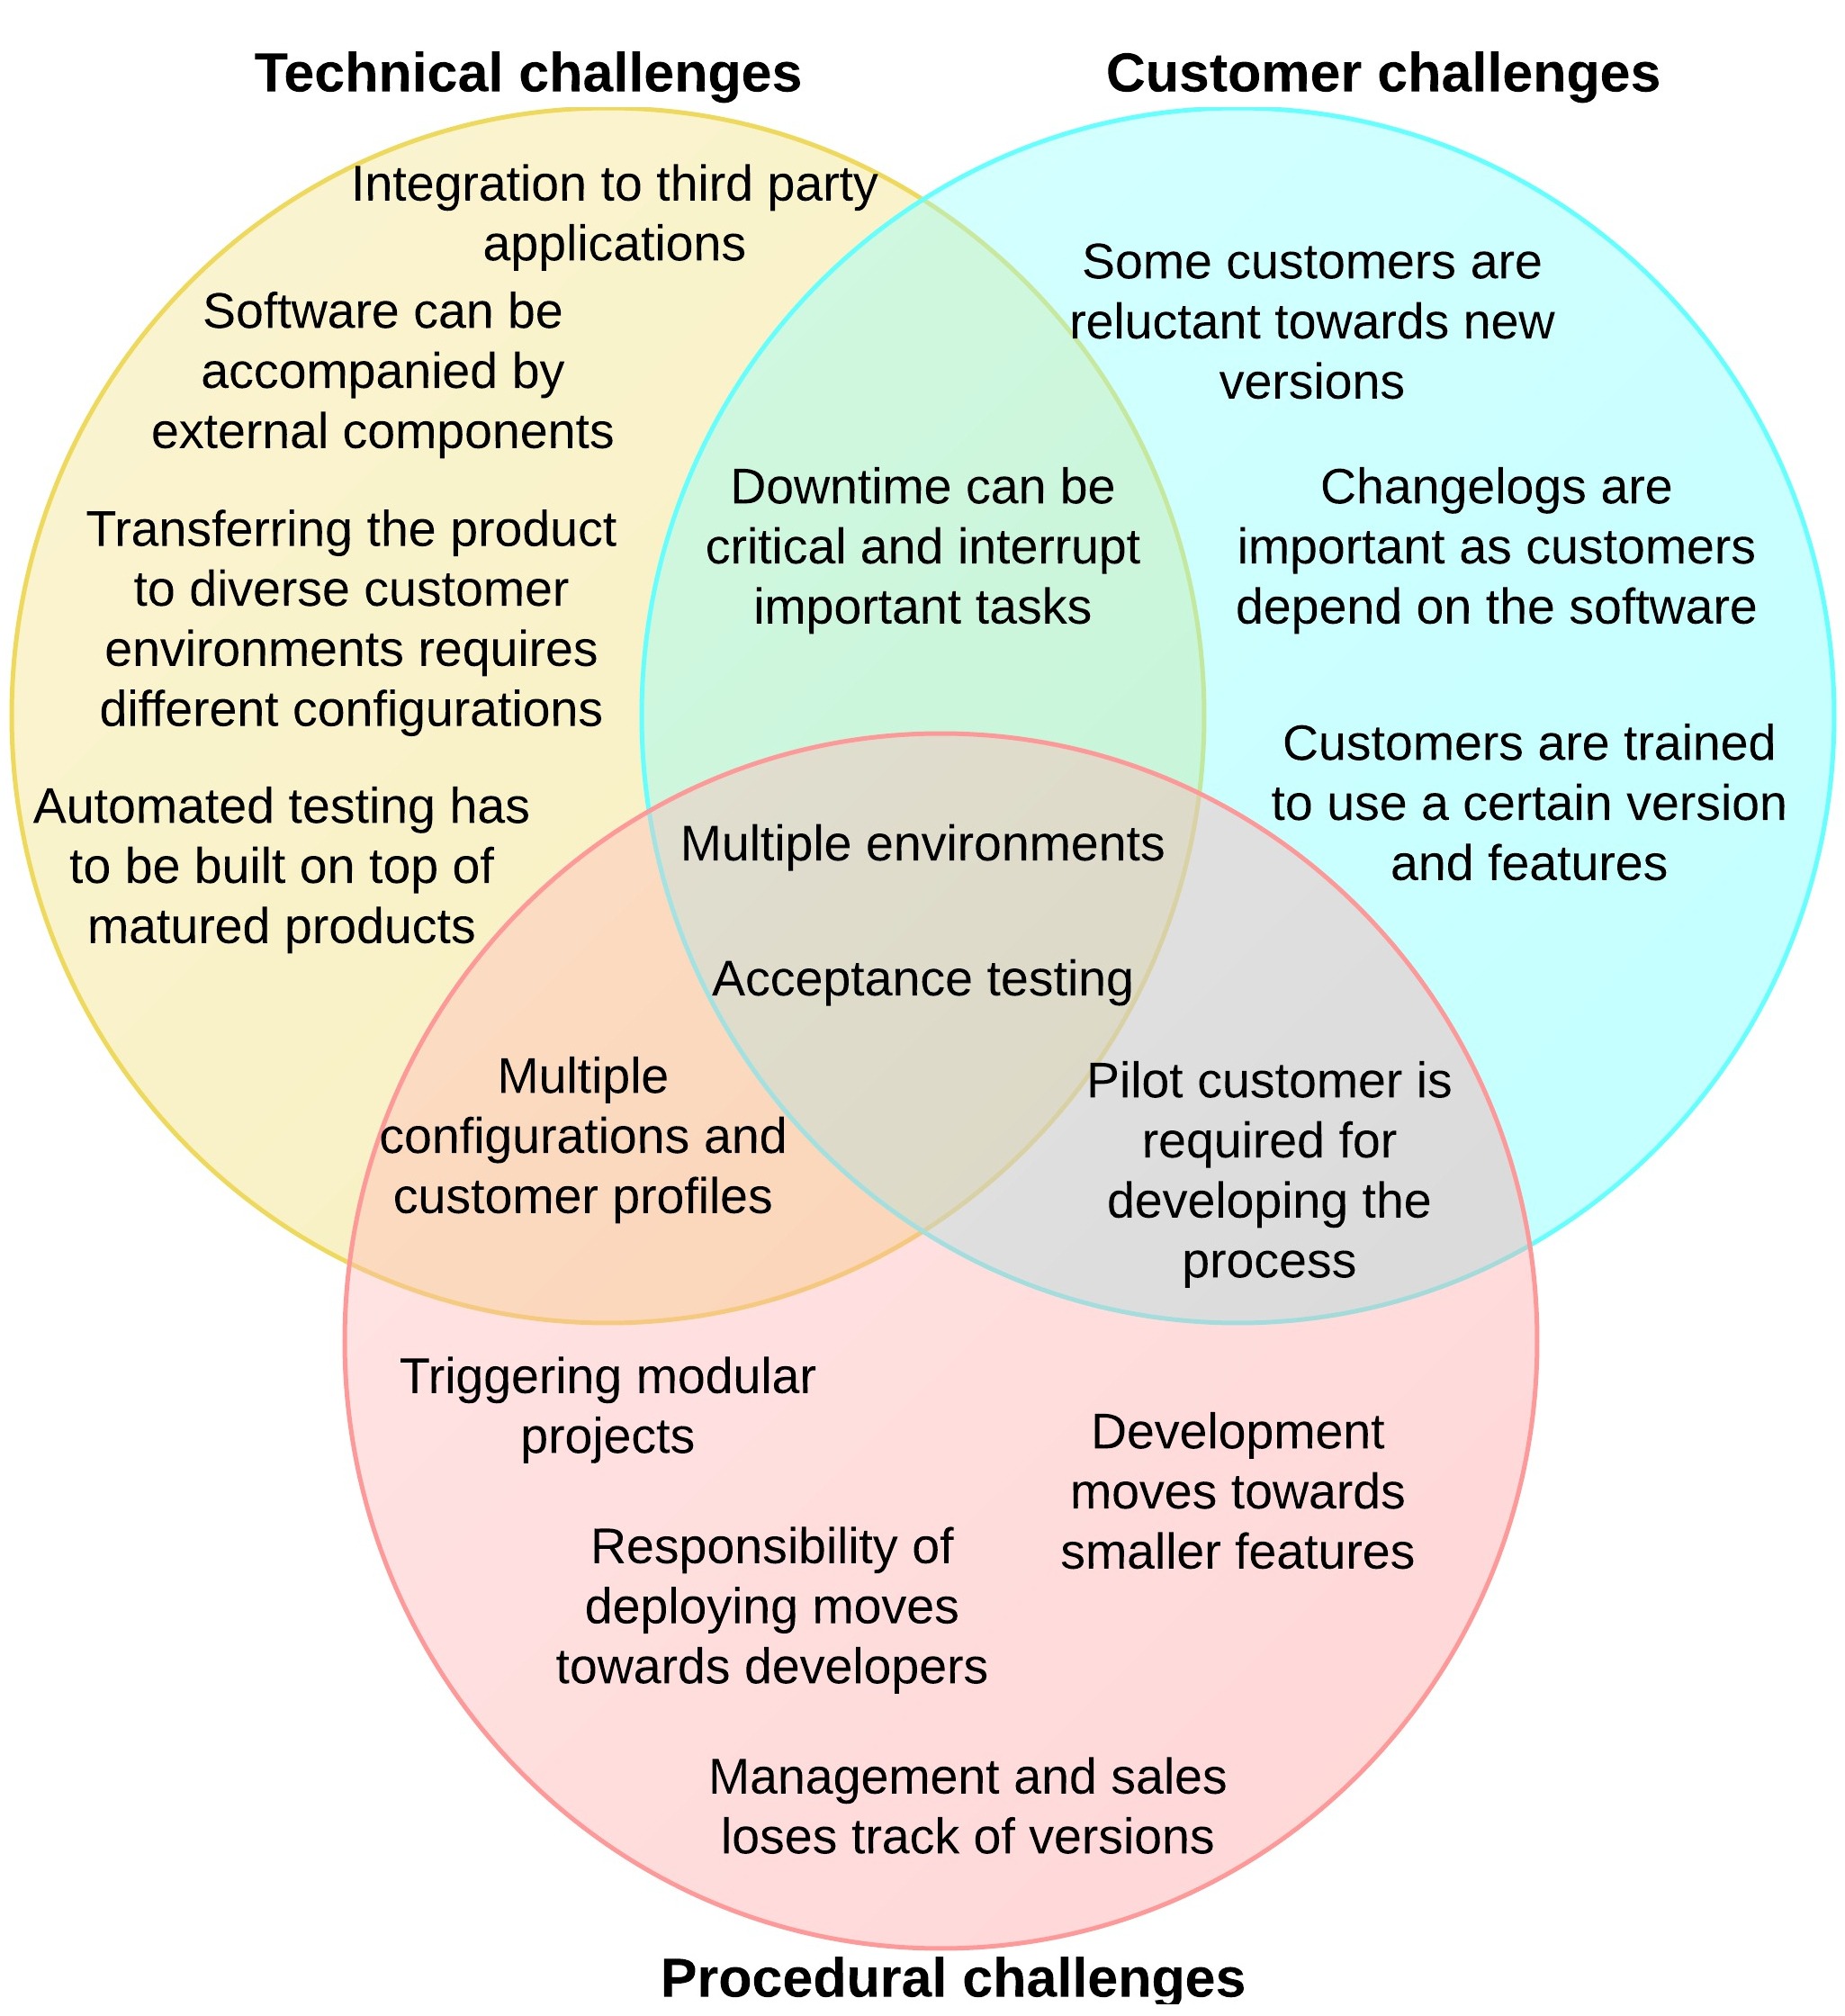
\includegraphics[width=5.0in]{cd_challenges.jpeg}
  \caption{Case company's challenges in continuous delivery.}
  \label{fig8}
\end{figure}

Fig. \ref{fig8} visualizes the challenges the case company faces in transition towards continuous delivery. Multiple challenges are related to two or more aspects, and the problems affecting all aspects can be seen as the core challenges. Acceptance testing is related to all aspects since customers want to perform acceptance testing with new versions, automated acceptance testing has to be implemented and the user acceptance testing is required before a production release can be made. Another challenge related to all aspects is the diversity of customer environments. It affects the technical implementation, as software has to be transferred to diverse environments. The procedural challenge is that the software has to be deployed multiple customers, and it has to be decided whether each version is always released to every customer. 

%to theory
The findings are in align with and could be considered as extending some of the theoretical contributions by Olsson et al. \cite{olsson2012climbing}, who researched the transition towards continuous delivery and an experimentational system. Identifying that transitioning towards continuous delivery requires a company to address issues in multiple aspects of the company also benefits companies in practice.   



\section{Summary}
This study was motivated by the general increased interest towards innovative experimental systems \cite{olsson2012climbing}, and the lack of related studies in the B2B domain. While especially continuous delivery and partly continuous experimentation have been utilized and researched in the B2C domain \cite{neely2013continuous, bosch2012building}, the benefits and challenges are still vague for B2B companies. Understanding the central aspects of continuous delivery and continuous experimentation will be a must for software companies willing to stay ahead of its competitors in the current rapidly moving industry.
%This study applied an exploratory view on the development model of the case company, deconstructing it into smaller parts. 

The focus of this study was not solely on the technical aspects of these development processes, as research already exists on these subjects \cite{kohavi2007practical, eklund2012architecture, cdbook}. Rather, the study focused on identifying the challenges in the transition towards these processes as a whole. The analysis of continuous delivery and continuous experimentation proceeded from higher-level considerations of requirements and benefits towards more detailed focus of applying continuous experimentation in B2B context. The findings provide insights into the challenges a company faces in the transition in this domain. In addition, the findings also compare the development models from the viewpoint of two different software products, providing further analysis on software product characteristics that affect these models.

This study has identified the main requirements a company operating in the B2B domain has to address when applying continuous delivery and continuous experimentation. In the case of continuous delivery, the challenges can be divided into technical challenges, procedural challenges and challenges related to the customer. These challenges are mostly caused by having multiple customers with diverse environments and unique properties, whose business depends on the software product. While continuously deploying versions to a user acceptance testing environment requires a company to address multiple challenges, continuously deploying to production is even more difficult. The reason for this is that some customers want to perform manual acceptance testing before production releases can be made. 

%The second research question answer
The benefits of these practices matched to many problems found in the case company, and a company operating in similar domain with similar products can use them as a basis when considering applying these practices. The most important challenges in the case company were found to be related to the deployment process and guiding the development of the software products. By utilizing continuous delivery, the case company can solve problems such as long feedback cycles, low reliability in new versions and high amount of resources required for releases. 


\subsection{Limitations}
Since case studies only allow analytic generalisations instead of statistical generalisations, the findings cannot be directly generalised to other cases. This limitation applies especially to results from first two research questions, which mostly rely on the qualitative data found from interviews. Limiting direct generalisation also applies to applying continuous experimentation in practice, since software products and customers inevitably differ. 

Two types of triangulation were used: data triangulation by including persons with different roles into the interviews, and methodological triangulation by collecting documentary data and observations by the author. However, the reliability of the results could have been increased by employing observer triangulation and theory triangulation. 

Regardless of the limitations a case study has, the phenomena was deeply understood through gathering a large amount of qualitative data and systematically analysing it. %utilize theoretical lens? 
Therefore the core findings should be applicable to similar research problems outside of the empirical context of this study. This means that the B2B challenges and benefits of continuous delivery and continuous experimentation can be considered as a starting point for further studies in other contexts where these development models take place.

The scope was limited to the development process of two software products within the case company, and direct generalisations to other domains and products should be avoided. However, the findings of this study are in align with and could be considered as extending some of the theoretical contributions by Olsson et al. \cite{olsson2012climbing}, who researched the transition from agile development towards an experimental system. 

While the data collection was applied to the teams developing the software products, the upper management of the company were not interviewed. The variety of responses in other teams was not explored, or the multitude of other different possible contexts in software development in the B2B domain. The responses from the interviewees mostly differentiated only based on the software product being developed, and the teams were quite similar in terms of composition and experience.
\subsection{Future research}
The individual aspects where challenges were found could be more deeply analyzed for both continuous delivery and continuous experimentation. Also, grouping the challenges into different groupings can yield interesting results. In the case of continuous experimentation, researching dependencies between problems in different groups could yield interesting results by providing a detailed view on the core challenges.

An interesting research question for further research is also how the core findings of the study can be transferred to other companies working in the B2B domain with different software products. This includes investigating deviations found in the challenges and benefits presented in this study. The challenges found in the transition phases also have to be validated by adopting the respective development model in practice. 

\paragraph{Notes and Comments.}
asd

%
% ---- Bibliography ----
%
\begin{thebibliography}{5}

\bibitem{smit:wat} Smith, T.F., Waterman, M.S.: Identification of Common Molecular
Subsequences. J. Mol. Biol. 147, 195--197 (1981)

\bibitem{mes} May, P., Ehrlich, H.C., Steinke, T.: ZIB Structure Prediction Pipeline:
Composing a Complex Biological Workflow through Web Services. In: Nagel,
W.E., Walter, W.V., Lehner, W. (eds.) Euro-Par 2006. LNCS, vol. 4128,
pp. 1148--1158. Springer, Heidelberg (2006)

\bibitem{fos:kes} Foster, I., Kesselman, C.: The Grid: Blueprint for a New Computing
Infrastructure. Morgan Kaufmann, San Francisco (1999)

\bibitem{cff} Czajkowski, K., Fitzgerald, S., Foster, I., Kesselman, C.: Grid
Information Services for Distributed Resource Sharing. In: 10th IEEE
International Symposium on High Performance Distributed Computing, pp.
181--184. IEEE Press, New York (2001)

\bibitem{fos:kes:2} Foster, I., Kesselman, C., Nick, J., Tuecke, S.: The Physiology of the
Grid: an Open Grid Services Architecture for Distributed Systems
Integration. Technical report, Global Grid Forum (2002)

\bibitem{url} National Center for Biotechnology Information, http://www.ncbi.nlm.nih.gov

\end{thebibliography}
%
\end{document}
